\documentclass[12pt]{article}
\usepackage[left=2cm,right=2cm,top=2cm,bottom=2cm,bindingoffset=0cm]{geometry}
\usepackage{fontspec}
\usepackage{polyglossia}
\usepackage{amssymb}
\setdefaultlanguage{russian}
\setmainfont[Mapping=tex-text]{CMU Serif}

\begin{document}
\centering {\LARGE Формальные языки}

{\Large домашнее задание до 23:59 21.09}
\bigskip

\enumerate
{
  \item
  {
    Перечислить слова языка $L_1 \cap L_2,$ где $L_1 = \{ (ab)^n \mid n \geq 0 \}$ и $L_2 = \{ a^m b^m \mid m \geq 0 \}$. Доказать, что других цепочек в пересечении нет. 
  }
  \item 
  { 
    Построить детерминированные \textbf{полные} конечные автоматы (если надо, добавить ``дьявольскую'' вершину) и представить описание в виде множества для следующих языков над алфавитом $\Sigma = \{ a, b, c \}$:
    \begin{enumerate}
        \item каждое слово языка содержит подслово $abb$ или $aac$;
        \item все слова начинаются и заканчиваются на одну и ту же букву;
        \item  буква $b$ не встречается ``правее'' буквы $a$ ни в одном слове
    \end{enumerate}
  }
  \item
  {
    Прочитать про алгоритмы минимизации и детерминизации на слайдах, прогнать их на примерах со следующих страниц этого документа, убедиться в собственном понимании алгоритмов. (не оценивается, но полезно) 
  }
  
  
\newpage
\begin{center} \Large{Пример применения алгоритма минимизации}
\end{center}

\bigskip

Минимизируем данный автомат:

\begin{center} 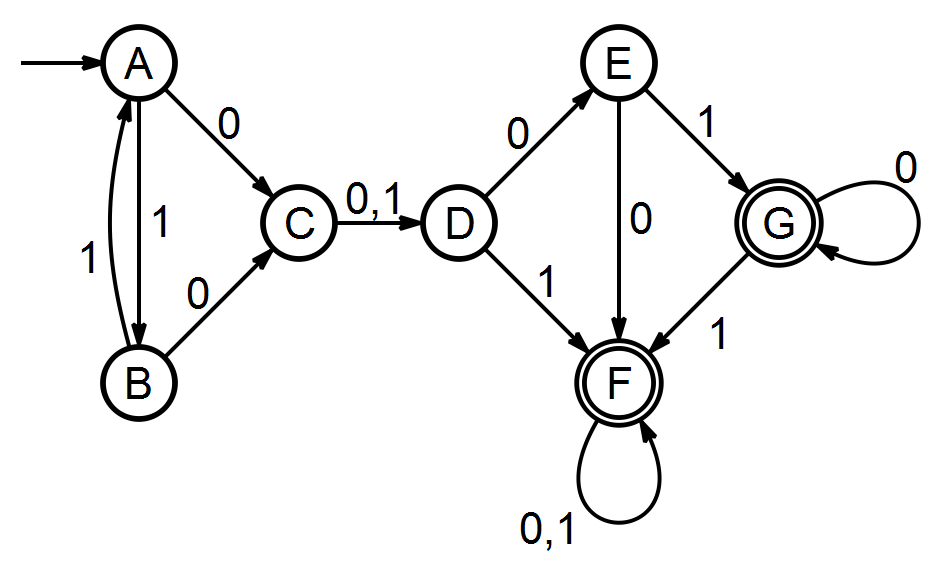
\includegraphics[width=0.65\linewidth]{../../2016_win/ElTech/2exmin.png} \end{center}

Автомат полный, в нем нет недостижимых вершин --- продолжаем.

Строим обратное $\delta$ отображение. 

\begin{tabular}{c|c|c}
$\delta^{-1}$ & 0 & 1 \\ \hline
A & --- & B \\
B & --- & A \\
C & A B & --- \\
D & C & C \\
E & D & --- \\
F & E F & D F G \\
G & G & E 
\end{tabular}

Отмечаем в таблице и добавляем в очередь пары состояний, различаемых словом $\varepsilon$: все пары, один элемент которых --- терминальное состояние, а второй --- не терминальное состояние. Для данного автомата это пары 

$(A, F), (B, F), (C, F), (D, F), (E,F), (A, G), (B, G), (C, G), (D, G), (E, G)$

Дальше итерируем процесс определения неэквивалентных состояний, пока очередь не оказывается пуста. 

$(A, F)$ не дает нам новых неэквивалентных пар. Для $(B, F)$ находится 2 пары: $(A, D), (A, G)$. Первая пара не отмечена в таблице --- отмечаем и добавляем в очередь. Вторая пара уже отмечена в таблице, значит, ничего делать не надо. Переходим к следующей паре из очереди. Итерируем дальше, пока очередь не опустошится. 

Результирующая таблица (заполнен только треугольник, потому что остальное симметрично) и порядок добавления пар в очередь.

\begin{tabular}{c|cc|cc|cc|c}
& A & B & C & D & E & F & G \\ \hline
A &&&&&&& \\
B &&&&&&& \\ \hline
C & \checkmark & \checkmark &&&&& \\
D & \checkmark & \checkmark & \checkmark &&&& \\ \hline
E & \checkmark & \checkmark & \checkmark & \checkmark &&& \\
F & \checkmark & \checkmark & \checkmark & \checkmark & \checkmark && \\ \hline
G & \checkmark & \checkmark & \checkmark & \checkmark & \checkmark && \\
\end{tabular}

Очередь: 

$
(A, F), (B, F), (C, F), (D, F), (E,F), (A, G), (B, G), (C, G), (D, G), (E, G),
$

$
(B, D), (A, D), (A, E), (B, E), (C, E), (C, D), (D, E), (A,C), (B, C))
$

В таблице выделились классы эквивалентных вершин: $\{A, B\}, \{C\}, \{D\}, \{E\}, \{F,G\}$. Остается только нарисовать результирующий автомат с вершинами-классами. Переходы добавляются тогда, когда из какого-нибудь состояния первого класса есть переход в какое-нибудь состояние второго класса. Минимизированный автомат: 

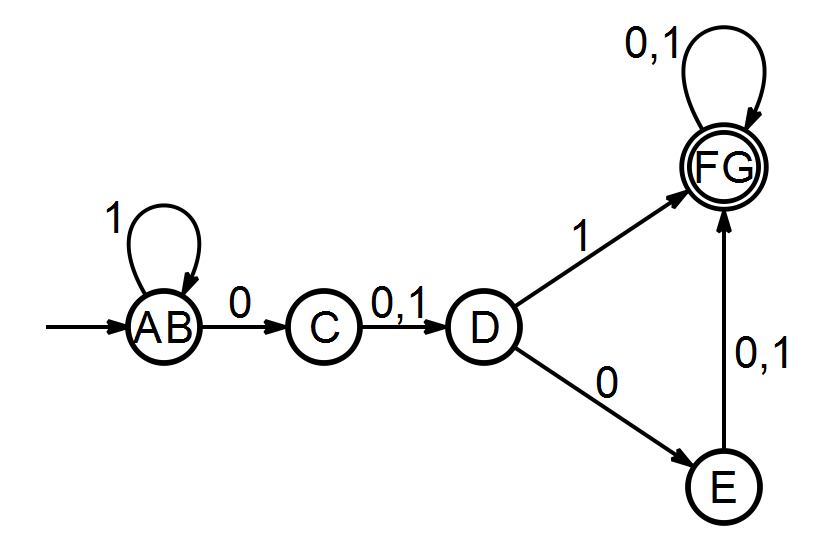
\includegraphics[width=0.65\linewidth]{../../2016_win/ElTech/2exminres.png}

\newpage

\begin{center} \Large{Пример применения алгоритма Томпсона}
\end{center}

\bigskip

Детерминизируем данный автомат: 

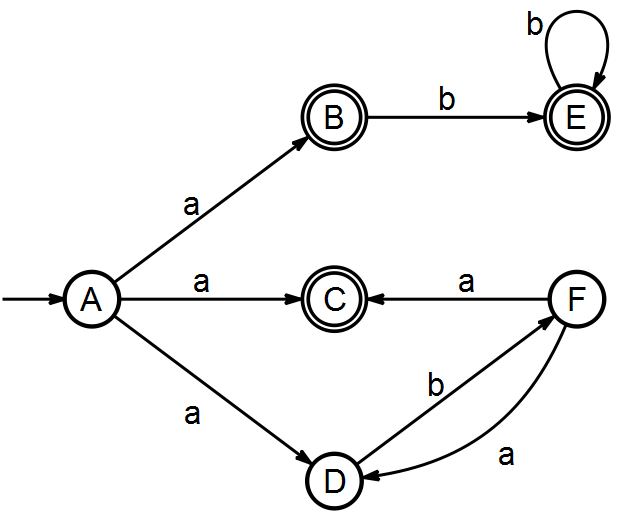
\includegraphics[width=0.65\linewidth]{../../2016_win/ElTech/2exdet.png}

Начинаем со стартового состояния. $\delta(A, a) = \{B, C, D\}; \delta(A, b) = \emptyset$. Добавляем вершину $\{B, C, D\}$, смотрим на переходы из нее: $\delta(B, b) = \{E\}; \delta(C, b) = \emptyset; \delta(D, b) = \{ F\}$. Объединяем результаты, получаем новое состояние $\{ E, F\}$ и переход $\delta'(\{B,C,D\}, b) = \{E, F\}$. Повторяем процедуру, пока не исследуем все переходы. Стартовое состояние --- множество из одного стартового состояния; терминальные состояния --- те, в которые попало хотя бы одно терминальное состояние исходного НКА.

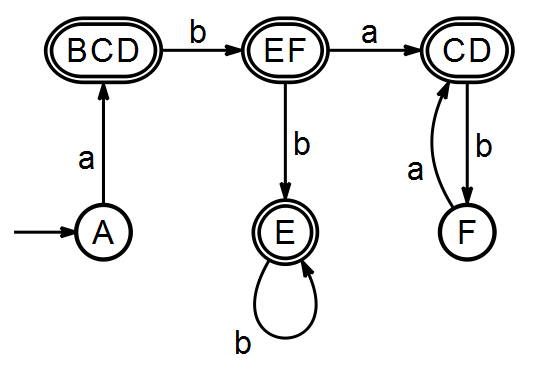
\includegraphics[width=0.65\linewidth]{../../2016_win/ElTech/2exdetres.png}



}
\end{document}
